% ===========================================================================
%  EndCorelib user guide
%
%  Build:   tectonic doc/userguide.tex       (or xelatex / lualatex / pdflatex,
%                                             run twice, from inside doc/)
%
%  Every program output in this guide is read from doc/out/, which
%  src/doc/run_examples.sh and src/doc/compare_options.sh regenerate from the code;
%  the figures come from src/doc/make_figures.py and the tables of Section 6 from
%  src/doc/make_tables.py.
% ===========================================================================
\documentclass[11pt,a4paper]{article}

\usepackage{iftex}
\ifPDFTeX
  \usepackage[T1]{fontenc}
  \usepackage{lmodern}
\else
  \usepackage{fontspec}
\fi
\usepackage[a4paper,margin=2.5cm]{geometry}
\usepackage{amsmath,amssymb}
\usepackage{xcolor}
\usepackage{fancyvrb,fvextra}
\usepackage{booktabs}
\usepackage{graphicx}
\usepackage{enumitem}
\usepackage{caption}
\usepackage{microtype}
\usepackage[hidelinks]{hyperref}

\definecolor{rule}{gray}{0.75}
\fvset{fontsize=\small,frame=leftline,framerule=0.6pt,rulecolor=\color{rule},
       framesep=0.8em,xleftmargin=1.2em,breaklines,breakanywhere=false}
% program output, in a smaller font so that the long lines fit
\newcommand{\out}[2][]{\VerbatimInput[fontsize=\footnotesize,#1]{#2}}

\newcommand{\file}[1]{\nolinkurl{#1}}
\newcommand{\eps}{\varepsilon}
\newcommand{\End}{\mathrm{End}}
\newcommand{\BoxOp}{\mathrm{Box}}
\newcommand{\wmax}{w_{\max}}

\setlist{itemsep=2pt,topsep=4pt}
\captionsetup{font=small,labelfont=bf}
\setlength{\parskip}{3pt}

\title{EndCorelib user guide\\[4pt]
       \large End covers for the initial value problem}
\author{Bingwei Zhang \and Chee Yap}
\date{November 2026}

\begin{document}
\maketitle

\tableofcontents

% ---------------------------------------------------------------------------
\section{What EndCorelib computes}
% ---------------------------------------------------------------------------

EndCorelib takes an autonomous system of ordinary differential equations
\[
  x' = f(x), \qquad x \in \mathbb{R}^n,
\]
a box $B_0 \subset \mathbb{R}^n$ of initial values, a horizon $H > 0$ and an
error bound $\eps > 0$. It returns a finite set $C$ of boxes with
\begin{equation}\label{eq:cover}
  \End(B_0,H) \;\subseteq\; \bigcup C \;\subseteq\; \End(B_0,H) + [-\eps,\eps]^n ,
\end{equation}
where $\End(B_0,H) = \{\, x(H) : x(0) \in B_0 \,\}$ is the set of states
reached at time $H$. A set $C$ with this property is an \emph{$\eps$-cover}
of the end set. The left inclusion says that no solution starting in $B_0$ is
lost. The right one holds because every box of $C$ is at most $\eps$ wide and
contains a point of the end set. All arithmetic is interval arithmetic with
directed rounding, so the inclusions hold for the boxes the program prints,
rounding errors included. If double precision runs out first, that is, if
Refine has not reached $\eps$ when $E_0$ can no longer be halved, the wider
box is kept, so that nothing is lost, and the program prints a note saying
so.

With most validated solvers you learn the width of the result after the run.
Here $\eps$ is an input: EndCorelib subdivides $B_0$ until every piece has an
end-enclosure at most $\eps$ wide, and $C$ is the set of these
end-enclosures. The program also reports $B_1 = \BoxOp(C)$, the smallest box
that contains the cover. Because every box of $C$ lies within $\eps$ of the
end set, $B_1$ exceeds the smallest box around $\End(B_0,H)$ by at most
$\eps$ on each side.

The cover can be much smaller than $B_1$. Figure~\ref{fig:eij} shows
Eijgenraam's example $x' = 0$, $y' = x^2$ with $x(0) \in [-1,1]$ and
$y(0) = 0$. At $H = 1$ the end set is the arc $y = x^2$, $|x| \le 1$. Every
convex set that contains the arc also contains $(0,1)$, the midpoint of its
two end points, although no solution comes near that point. The cover for
$\eps = 0.1$ has 40 boxes and follows the arc.

\begin{figure}[htb]
  \centering
  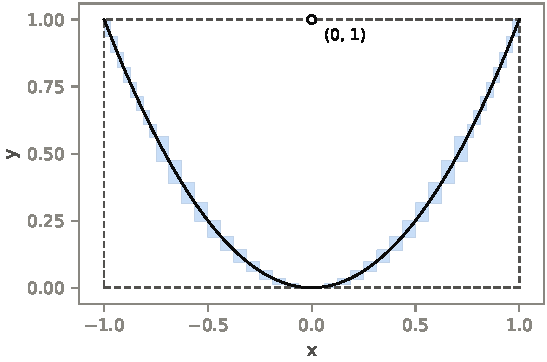
\includegraphics[width=0.62\textwidth]{fig/eijgenraam.pdf}
  \caption{Eijgenraam's example at $H=1$: the $0.1$-cover (40 boxes), the
    end set $y = x^2$ (black) and the bounding box $B_1$ of the cover
    (dashed). The point $(0,1)$ lies in $B_1$ and in every convex enclosure
    of the arc. Data from \texttt{make run EG=src/examples/fig1Eijgenraam.mk}.}
  \label{fig:eij}
\end{figure}

The algorithm is the one of B.~Zhang and C.~Yap, \emph{End Cover for Initial
Value Problem: Complete Validated Algorithm with Complexity Analysis}
(arXiv:2502.00503 and arXiv:2602.00162), called \emph{the paper} below.
Section and equation numbers such as (5.5) refer to it.
Section~\ref{sec:code} shows where each part of the paper sits in the code.
Everything runs in IEEE double precision.

% ---------------------------------------------------------------------------
\section{Installing}\label{sec:install}
% ---------------------------------------------------------------------------

\subsection{What you need}

\begin{itemize}
  \item A C++17 compiler: g++ 9 or newer, or clang++ 10 or newer.
  \item GNU make and bash, for the Makefile and the scripts in
        \file{src/repro/} and \file{src/doc/}. CMake 3.16 or newer if you
        prefer the CMake build.
  \item CAPD (\url{http://capd.ii.uj.edu.pl}), which supplies the interval
        arithmetic and the Taylor coefficients of $f$.
  \item Optional: SymEngine, which multiplies out the right-hand side before
        it is evaluated (Section~\ref{sec:form}); Python~3 with matplotlib for
        the plots; MATLAB for \file{src/tools/pendulum_ode45.m} only.
\end{itemize}

On Windows, install Cygwin with the packages \texttt{gcc-g++}, \texttt{make},
\texttt{cmake} and \texttt{git}, and type every command of this guide in a
Cygwin login shell. Build EndCorelib in the same shell that built CAPD. Inside
Cygwin the Windows path \verb|C:\Users\you\CAPD| is written
\file{/cygdrive/c/Users/you/CAPD}.

\subsection{Building CAPD}

Clone CAPD wherever you like and build it; you will need the path in the
next step.
\begin{Verbatim}
cd ~
git clone https://github.com/CAPDGroup/CAPD.git
cd CAPD && mkdir build && cd build
cmake .. -DCMAKE_BUILD_TYPE=Release -DCAPD_BUILD_EXAMPLES=OFF -DCAPD_BUILD_TESTS=OFF
make -j4
\end{Verbatim}
This leaves \file{libcapd.a} in \file{~/CAPD/build}. Running
\verb|make install| is optional.

\subsection{Building EndCorelib}

EndCorelib reads the location of CAPD from a file \file{config.mk} in its top
directory. Copy the template and change its one active line to the absolute
path of the directory you cloned CAPD into (the one that contains
\file{capdDynSys/} and \file{build/}):
\begin{Verbatim}
cp config.mk.example config.mk
# in config.mk:
CAPD_MASTER := /home/you/CAPD
\end{Verbatim}
\file{config.mk} is ignored by git, so the path stays on your machine. You
can also give the path on each call, \verb|make CAPD_MASTER=/home/you/CAPD|,
or point at an installed CAPD with
\verb|make CAPD_CONFIG=/usr/local/bin/capd-config|. If \texttt{capd-config}
is on your \texttt{PATH}, a plain \texttt{make} finds it.

Now run \texttt{make}. The first line it prints names the CAPD it uses and
the last one is \texttt{Built EndCorelib}. If it says \texttt{CAPD not found},
check that \file{build/libcapd.a} exists under the directory you gave. Three
companion programs are built on request: \texttt{make EndCoretraj}, a
validated trajectory printer used by \texttt{make verify};
\texttt{make capdref}, the plain CAPD integrator behind the CAPD rows of the
paper's Table~2; and \texttt{make EndCoreaudit}, the box-by-box check of
Section~\ref{sec:repro}. \texttt{make tools} builds all three.

There is also a CMake build:
\begin{Verbatim}
mkdir build && cd build
cmake .. -DCMAKE_BUILD_TYPE=Release
cmake --build . --parallel
ctest
\end{Verbatim}
It uses \texttt{capd-config} when it finds one and otherwise downloads CAPD
from GitHub and builds it first. SymEngine is used only with
\verb|-DUSE_SYMENGINE=ON|. Both builds compile with
\verb|-frounding-math|. Keep it: without it the compiler may assume
round-to-nearest and break the directed rounding that every interval bound
relies on.

CAPD can be built with the interval type of the filib library, which its
CMake build does by default, or with its own interval type. EndCorelib uses
only operations that both provide and compiles against either.

\subsection{Checking the build}

\texttt{make check} runs 18 short computations and compares $B_1$, rounded to
two decimals, and the number of boxes $\#(C)$ with stored values. It takes
about fifteen seconds and should end like this:
\out[firstline=24]{out/check.txt}
The stored values hold whether or not SymEngine was found
(Section~\ref{sec:form} explains why that could matter).

% ---------------------------------------------------------------------------
\section{A first run}\label{sec:first}
% ---------------------------------------------------------------------------

\subsection{An example from the paper}

The directory \file{src/examples/} holds the test problems of the paper's
Table~1 as \file{.mk} files. Eg1 is the Lotka-Volterra system
$x' = 2x(1-y)$, $y' = -y(1-x)$ from $B_0 = [0.9,1.1]\times[2.9,3.1]$, with
$H = 4$ and $\eps = 1$ in the file:
\out{out/quickstart.txt}
In the examples of this guide a line that starts with \verb|$| is what was
typed; the lines below it are what the program printed. Reading the output
from the top:
\begin{description}[font=\ttfamily\mdseries,leftmargin=2em,style=nextline]
  \item[EndCorelib mode=\dots] the settings in force. The file says
        \texttt{tubedegree=0}, which selects the Euler tube, printed as
        \texttt{tubedegree=1}.
  \item[f =] the right-hand side in the form in which it is evaluated
        (Section~\ref{sec:form}).
  \item[B0, H, eps] the initial box, the horizon and $\eps$.
  \item[time(ms)] the wall-clock time of the computation in milliseconds.
  \item[Hull(T=4.000000)] the box $B_1 = \BoxOp(C)$, as one interval per
        coordinate.
  \item[B1] the same box as midpoint $\pm$ half-width, the form of the
        $B_1$ column of the paper's Table~2.
  \item[wmax(B1)] the largest side of $B_1$.
  \item[\#(C)] the number of boxes in the cover. \texttt{\#E0} counts the
        sub-boxes of $B_0$ that were integrated, one for each box of $C$, and
        the last number is the largest side among the boxes of $C$, which is
        at most $\eps$.
\end{description}
Here $C$ has 2 boxes, none wider than 0.799, and $B_1$ is 0.932 wide in $x$
and 0.133 wide in $y$.

\subsection{The same run without make}

\texttt{make} passes the fields of the \file{.mk} file to the program as
positional arguments. \texttt{make show-args} prints the command instead of
running it:
\out{out/showargs.txt}
The quotes are only there for the shell. Typed by hand, the same run is
\out[lastline=1]{out/cli_eg1.txt}
and it prints the same lines as \texttt{make run-eg1Volterra}.
Table~\ref{tab:args} lists the arguments in order.
Section~\ref{sec:options} discusses how to choose them, and the program
prints a short summary when it is called without arguments
(Appendix~\ref{app:usage}).

\begin{table}[htb]
\centering\small
\caption{The command-line arguments of \texttt{EndCorelib}, in order.}
\label{tab:args}
\begin{tabular}{lp{0.7\textwidth}}
\toprule
argument & meaning \\
\midrule
\texttt{output\_mode} & how much is printed and written, 0 to 4
                        (Table~\ref{tab:levels}) \\
\texttt{mode}         & 0: EndCover, cover all of $B_0$; 1: Boundary, cover
                        only the boundary of $B_0$ \\
\texttt{method}       & the refinement operators Refine may use: 0
                        \texttt{tube}, 1 \texttt{bisect}, 2
                        \texttt{splitonly} \\
\texttt{stepB}        & the one-step enclosure: 0 \texttt{lohner}, 1
                        \texttt{lohner+lognorm}, 2 \texttt{lohnerHO+lognorm},
                        3 \texttt{lohnerHO} \\
\texttt{tubedegree}   & 0 or 1, both the Euler tube of the paper's
                        Section 5.2; no other value is accepted \\
\texttt{n}            & the dimension $n$ \\
\texttt{var\_1 \dots\ var\_n} & the names of the variables \\
\texttt{f\_1 \dots\ f\_n}     & the right-hand sides (Section~\ref{sec:rhs}) \\
\texttt{eps}          & the error bound $\eps > 0$ \\
\texttt{order}        & the Taylor order of StepB, at least 3; the paper
                        uses 20 \\
\texttt{T}            & the horizon $H > 0$ \\
\texttt{debug}        & progress reports, 0 to 3 (Section~\ref{sec:debug}) \\
\texttt{lo\_1 hi\_1 \dots\ lo\_n hi\_n} & the initial box $B_0$ \\
\bottomrule
\end{tabular}
\end{table}

\subsection{Output levels and files}

\texttt{output\_mode} is cumulative: each level prints what the levels below
it print and adds the items of Table~\ref{tab:levels}. Level 2 is the usual
choice. The files are written into the current directory, and every run
appends one line to \file{out.txt}.

\begin{table}[htb]
\centering\small
\caption{What each output level adds, and the files it writes.}
\label{tab:levels}
\begin{tabular}{lp{0.78\textwidth}}
\toprule
level & adds \\
\midrule
0 & \texttt{time(ms)} \\
1 & the header lines, \texttt{Hull}, \texttt{B1} and \texttt{wmax(B1)} \\
2 & \texttt{\#(C)}, \texttt{\#E0} and the largest side among the boxes of $C$ \\
3 & \file{E0.txt}: the sub-boxes of $B_0$ that were integrated, in the order
    of $C$; \file{E1.txt}: the cover $C$; in two dimensions
    \file{convex_hull.txt}, the convex hull of $C$ as a closed polygon \\
4 & \file{E_0.txt}, \file{E_1.txt}: the same, plus the images of every
    sub-box at $t = 0.1$, $0.4$ and $0.7$ and, in two dimensions, the
    trajectories of the four corners of $B_0$, for plotting \\
\bottomrule
\end{tabular}
\end{table}

Here is Eg1 again with $\eps = 0.1$ at level 3, followed by the first lines
of \file{E1.txt} and the last two lines of the log:
\out{out/files.txt}
\out{out/files_head.txt}
\out[tabsize=2,breakanywhere]{out/files_log.txt}
A box file has one box per line, \texttt{Box k: [lo, hi] x [lo, hi] \dots},
with 17 significant digits; line $k$ of \file{E0.txt} and line $k$ of
\file{E1.txt} belong together. The columns of \file{out.txt} are separated by
tabs and named in its first line. Figure~\ref{fig:eg1} draws the two box
files. To draw them yourself, run
\begin{Verbatim}
python3 src/tools/plot_boxes.py . --save cover.png
\end{Verbatim}
in the directory that holds them.

\begin{figure}[htb]
  \centering
  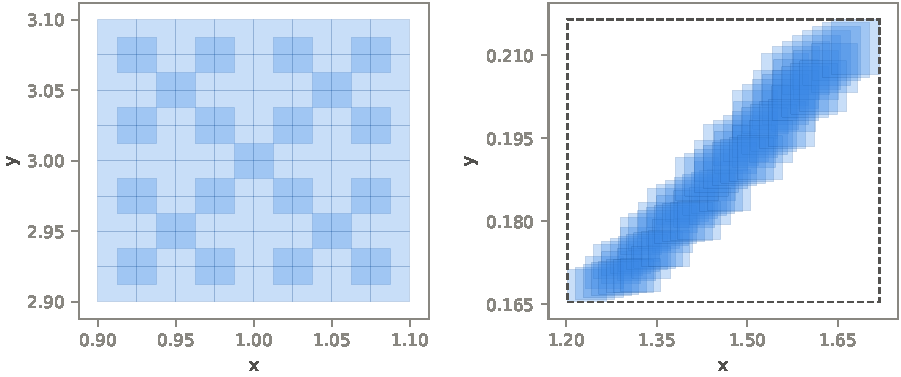
\includegraphics[width=\textwidth]{fig/eg1_cover.pdf}
  \caption{Eg1 with $\eps = 0.1$ and $H = 4$. Left: the 48 sub-boxes of
    $B_0$ in \file{E0.txt}. Right: the 48 boxes of the cover $C$ in
    \file{E1.txt} and their bounding box $B_1$ (dashed).}
  \label{fig:eg1}
\end{figure}

The 48 boxes of \file{E0.txt} tile $B_0$: 32 are squares of side 0.025, and
16 are 0.05 wide in $x$ and 0.025 in $y$. Each is the $E_0$ of one scaffold,
obtained from $B_0$ by \texttt{Split}, which halves a longest side, and line
$k$ of \file{E1.txt} is its end-enclosure at $H$.

% ---------------------------------------------------------------------------
\section{A problem of your own}\label{sec:own}
% ---------------------------------------------------------------------------

\subsection{A \texttt{.mk} file}

Take the damped pendulum $x' = y$, $y' = -\sin x - 0.2\,y$ from the box
$[0.9,1.1]\times[-0.1,0.1]$ up to $H = 10$. The file
\file{src/examples/dampedPendulum.mk} describes it:
\VerbatimInput[fontsize=\footnotesize]{../src/examples/dampedPendulum.mk}
\texttt{var} and \texttt{ff} are comma-separated lists. \texttt{cen} and
\texttt{wid} give the box as centre and half-width in each coordinate;
\verb|lohi = "0.9 1.1 -0.1 0.1"| would give it by its bounds instead. The
other fields are the arguments of Table~\ref{tab:args}, and
\file{src/examples/_template.txt} describes them all. Run the file with
\texttt{make run}:
\out{out/pendulum.txt}
Any field can be set on the command line without editing the file. Here
$\eps$ is halved and the progress reports of Section~\ref{sec:debug} are
switched on:
\out{out/pendulum_debug.txt}

\subsection{Writing the right-hand side}\label{sec:rhs}

An $f_i$ may use \verb|+ - * /|, parentheses, powers \verb|x^3|, and the
functions \texttt{sin}, \texttt{cos}, \texttt{exp}, \texttt{log},
\texttt{sqrt}, \texttt{sqr}, \texttt{atan}, \texttt{asin} and \texttt{acos}.
A number directly followed by a name or an opening parenthesis is
multiplied by it, so \verb|2x| is \verb|2*x| and \verb|(x+1)(y-1)| is
\verb|(x+1)*(y-1)|; digits inside a name, as in \verb|x1| or \verb|k2a|,
belong to the name. In a \file{.mk} file the commas separate the $f_i$, so an
$f_i$ cannot contain one. On the command line each $f_i$ is a separate
argument: quote it when it contains parentheses or other characters the
shell would interpret,
\out[lastline=1]{out/sci.txt}

\subsection{Constants}\label{sec:const}

A decimal constant such as \verb|0.2| is read as the double nearest to it
and enters the computation as an interval of width zero. The cover is then
rigorous for the system whose coefficient is that double, which differs from
$0.2$ by about $10^{-17}$. If the coefficient is meant to be exactly $1/5$,
write \verb|1/5|: a quotient is evaluated in interval arithmetic and its
enclosure contains the exact value, and the same holds for \verb|8/3| in the
Lorenz example. Constants in scientific notation are turned into such
quotients, \verb|2e-1| into \verb|(2/10^1)|. The header of the run above
shows the result:
\out[firstline=2]{out/sci.txt}

\subsection{The form of the expression}\label{sec:form}

Interval evaluation depends on how an expression is written: $x(1-x)$ and
$x - x^2$ are the same function but give different enclosures over a box.
If SymEngine was found when EndCorelib was built, every $f_i$ is first
multiplied out into a sum of monomials, so that \verb|(1-x^2)*y-x| becomes
\verb|-x+y-x^2*y|. Without SymEngine it is evaluated as written. The
\verb|f =| line of the output shows the form that was used.

On Lorenz (Eg5) the difference shows in the work. Run to $H = 5$ with
$\eps = 1$ and \texttt{stepB=0}, written as
\verb|10*(y-x), x*(28-z)-y, x*y-8*z/3| and evaluated as written, EndCover
split $B_0$ down to depth 7, processed 116 scaffolds and returned 78 boxes.
Multiplied out, it stopped at depth 6 after 95 scaffolds and 64 boxes. The
files in \file{src/examples/} and the scripts in \file{src/repro/} therefore
spell out the multiplied-out form.
That is also the form the numbers of the paper were computed from, so these
files give the same results in builds with and without SymEngine.

\subsection{Mistakes in the input}

A wrong argument count, a negative $\eps$ or a box with \verb|lo > hi| stops
the program with \texttt{Argument error} and the usage summary. A right-hand
side that cannot be read is reported with the map string the parser was
given; here \verb|Y| should have been \verb|y|:
\out{out/parse_error.txt}
Both cases end with exit status 2.

% ---------------------------------------------------------------------------
\section{Following a long run}\label{sec:debug}
% ---------------------------------------------------------------------------

A run can take hours, and with \texttt{debug=0} it prints nothing until it
is finished. The \texttt{debug} argument switches on progress reports:

\begin{center}\small
\begin{tabular}{lp{0.75\textwidth}}
\toprule
\texttt{debug} & reports \\
\midrule
0 & none \\
1 & one line for every scaffold that EndCover has taken from its queue \\
2 & also one line for every scaffold laid out to the horizon and for every
    pass of Refine \\
3 & also one line for every stage appended by Extend, and the containment
    self-checks, which should never fire \\
\bottomrule
\end{tabular}
\end{center}

Each line starts with the wall-clock time since the program started. The
reports go to standard error and the results to standard output, so
\verb|> result.txt| still captures the results alone, and
\verb|2> progress.log| keeps the reports in a file you can follow with
\verb|tail -f progress.log|.

\subsection{One line per scaffold}

Eg1 with $\eps = 0.5$ at \texttt{debug=1}:
\out{out/debug1.txt}
Each scaffold taken from the queue gets one line, written when it is
finished:
\begin{description}[font=\ttfamily\mdseries,leftmargin=2em,style=nextline]
  \item[run] the number of the scaffold, in the order processed.
  \item[depth] how often $B_0$ was split to obtain its initial box $B$;
        $B_0$ itself has depth 0. \texttt{Split} halves a longest side, so
        in $n$ dimensions $\wmax(B)$ halves every $n$ levels.
  \item[wmax(E\_m)] the width of its end-enclosure at $H$.
  \item[queue] the scaffolds still waiting.
  \item[done] the share of $B_0$, by volume, that the cover already covers.
  \item[outcome] \texttt{resolved}: the scaffold reached $H$ with an
        end-enclosure at most $\eps$ wide, which goes into $C$.
        \texttt{resolved, E\_0 -> w, k split off}: on the way Refine called
        \texttt{Split} $k$ times, so $E_0$ ended at width $w$, and the $k$
        halves split off went into the queue as new scaffolds.
        \texttt{split:} the scaffold could not be carried to the
        horizon, for the reason given, and its initial box was split in two
        (Section~\ref{sec:fail}).
\end{description}
EndCover always takes the scaffold queued last, so it works depth first. In
this run Refine split $E_0$ twice in run 1, first along $x$ and then along
$y$, and the two halves it split off became runs 3 and 2; run 3 split once
more, and its half became run 4. The four end-enclosures form $C$, and the
four final $E_0$ tile $B_0$ with squares of side 0.1.

\subsection{Inside one scaffold}

At \texttt{debug=2} each scaffold also shows how it was built and refined:
\out[lastline=16]{out/debug2.txt}
\texttt{scaffold laid out} means that Extend has reached $t = H$ in $m$
stages; the widths of $E_0$ and of the end-enclosure $E_m$ follow.
\texttt{split-off scaffold evaluated} reports the same for a scaffold that
\texttt{Split} split off: it is a copy of the scaffold it came from, with
its own half as $E_0$, and is walked once from that half. Each
\texttt{Refine pass} line reports one pass of the main loop of Refine:
the new widths of $E_m$ and $E_0$; \texttt{mu\_max}, the logarithmic-norm
bound that enters the tests (5.4) and (5.5); the number of stages $m$; how
many stages \texttt{Bisect} refined in this pass; how many stages are frozen
by (5.4); and how many times \texttt{Split} halved $E_0$. For run 1, Extend
reached $H = 4$ in 55 stages with an end-enclosure 6.3 wide. Each of the two
passes of Refine bisected all 55 stages and split once, which brought $E_m$
down to 0.80 and then to 0.41, below $\eps = 0.5$. The half split off in the
second pass, run 2, was within $\eps$ as soon as it was evaluated, so Refine
had nothing to do.

At \texttt{debug=3} every stage appears as Extend appends it, with its end
time $t_i$, its length $h$ and its end-enclosure $E_i$:
\out[lastline=12]{out/debug3.txt}
Short stages mark the parts of $[0,H]$ where StepA or the error control of
StepB allowed only small steps.

\subsection{A long run}

Lorenz (Eg5) to $H = 5$ with $\eps = 1$, from the \file{.mk} file, begins
\out[lastline=10]{out/lorenz_T5.txt}
and ends
\out[firstline=96]{out/lorenz_T5.txt}
The scaffold of $B_0$ could not be carried past $t = 3.79$ and those of its
halves past $t = 3.95$; the boxes of depths 2, 3 and 4 got to $t = 4.43$,
$4.65$ and $4.69$. The 32 boxes of depth 5 reached $H = 5$, Refine split each
of them once more, and the 64 end-enclosures, all from boxes of depth 6, form
$C$; a scaffold that was split in two contributes nothing. The
\texttt{done} column moves by $1/64 \approx 1.6\%$ with each resolved
scaffold, so after a few minutes of a long run it tells you roughly how much
longer to wait.

% ---------------------------------------------------------------------------
\section{Choosing the options}\label{sec:options}
% ---------------------------------------------------------------------------

The inputs that decide what you get are $\eps$ and $H$. The other options
decide how the work is done, and on the problems of the paper most of them
change the time much more than the result. Every run below starts from the
settings of the example files
(\texttt{mode=0}, \texttt{method=0}, \texttt{stepB=0}, \texttt{tubedegree=0},
\texttt{order=20}), changes one option, and runs the problem to the longer
horizon of the paper's Table~2. The runs come from
\file{src/doc/compare_options.sh}, six at a time on an Intel Core i7-13700HX,
and \file{src/doc/make_tables.py} turned them into the tables, so both can be
regenerated. Times are wall-clock seconds. A run that was still going after
ten minutes was stopped; its cell shows $>$600 and has no result. Running
several at a time makes the times less precise, so read only the larger
differences in the tables, and compare times within a table rather than
with your own machine. The last table was measured two runs at a time.

\subsection{The error bound}

\begin{table}[htb]
\centering\small
\caption{Time and number of boxes as $\eps$ shrinks (all other options at
  their defaults).}
\label{tab:eps}
%% generated by src/doc/make_tables.py from doc/out/options/
\begin{tabular}{llrrrrrr}
\toprule
& & \multicolumn{2}{c}{$\varepsilon=1$} & \multicolumn{2}{c}{$\varepsilon=0.5$} & \multicolumn{2}{c}{$\varepsilon=0.1$} \\
\cmidrule(lr){3-4}\cmidrule(lr){5-6}\cmidrule(lr){7-8}
problem & $H$ & s & $\#(C)$ & s & $\#(C)$ & s & $\#(C)$ \\
\midrule
Eg1 Lotka-Volterra & 5.5 & 24 & 48 & 30 & 64 & 360 & 274 \\
Eg2 Van der Pol & 2 & 1.2 & 4 & 2.0 & 6 & 41 & 51 \\
Eg3 quadratic & 4 & 0.9 & 8 & 1.7 & 13 & 61 & 143 \\
Eg4 FitzHugh-Nagumo & 4 & 0.7 & 2 & 0.8 & 2 & 1.8 & 6 \\
Eg5 Lorenz & 4 & 55 & 8 & 74 & 8 & $>$600 & -- \\
Eg6 R\"ossler & 4 & 0.2 & 1 & 0.3 & 1 & $>$600 & -- \\
\bottomrule
\end{tabular}

\end{table}

Going from $\eps = 1$ to $\eps = 0.5$ at most doubled the number of boxes,
and left it unchanged on FitzHugh-Nagumo, Lorenz and R\"ossler
(Table~\ref{tab:eps}). From 0.5 to 0.1 the number of boxes grew by a factor of 2 to 12 where the runs
finished, and the time by a factor of up to 140; Lotka-Volterra, Lorenz and
R\"ossler did not finish within ten minutes. R\"ossler is the extreme case:
without any subdivision its end-enclosure is 0.495 wide, so $\eps = 0.5$
takes a fifth of a second. Every split halves one side of a box, so the cost
depends on how far $\eps$ lies below the width of the undivided
end-enclosure. Start with a generous $\eps$, look at $\#(C)$ and the time,
and lower it in steps.

\subsection{The horizon}

The horizon sets how far the end set has spread by the time the cover is
taken. For Lotka-Volterra with $\eps = 0.1$ and \texttt{method=2} the cover
has 56 boxes at $H = 4$ and 297 at $H = 5.5$. For a chaotic system the
horizon also decides whether a run can finish at all, because every level
of splitting doubles the work and gains only a fixed amount of time; Section~\ref{sec:fail} shows how to read that amount off the
progress report.

\subsection{The enclosure step: \texttt{stepB}}

\begin{table}[htb]
\centering\small
\caption{The four StepB variants: time and $\wmax(B_1)$.}
\label{tab:stepB}
%% generated by doc/make_tables.py from doc/out/options/
\begin{tabular}{lll rrrr rrrr}
\toprule
& & & \multicolumn{4}{c}{time (s) for \texttt{stepB}} & \multicolumn{4}{c}{$w_{\max}(B_1)$ for \texttt{stepB}} \\
\cmidrule(lr){4-7}\cmidrule(lr){8-11}
problem & $H$ & $\varepsilon$ & 0 & 1 & 2 & 3 & 0 & 1 & 2 & 3 \\
\midrule
Eg1 Lotka-Volterra & 5.5 & 0.5 & 18 & 29 & 23 & 8.2 & 1.074 & 1.074 & 0.967 & 0.967 \\
Eg2 Van der Pol & 2 & 0.5 & 1.6 & 2.7 & 2.8 & 0.9 & 0.715 & 0.715 & 0.685 & 0.685 \\
Eg3 quadratic & 4 & 0.5 & 1.2 & 2.3 & 2.5 & 0.9 & 0.861 & 0.861 & 0.858 & 0.858 \\
Eg4 FitzHugh-Nagumo & 4 & 0.5 & 1.1 & 1.4 & 0.2 & 0.1 & 0.170 & 0.170 & 0.207 & 0.207 \\
Eg5 Lorenz & 4 & 0.5 & 14 & 28 & 258 & 66 & 0.458 & 0.458 & 0.135 & 0.135 \\
Eg6 R\"ossler & 4 & 0.5 & 0.2 & 0.5 & 0.2 & 0.1 & 0.495 & 0.495 & 0.484 & 0.484 \\
\addlinespace
Eg1 Lotka-Volterra & 5.5 & 0.1 & 173 & 311 & 247 & 74 & 0.849 & 0.849 & 0.841 & 0.841 \\
Eg2 Van der Pol & 2 & 0.1 & 20 & 37 & 30 & 9.2 & 0.610 & 0.610 & 0.609 & 0.609 \\
Eg3 quadratic & 4 & 0.1 & 36 & 73 & 39 & 13 & 0.803 & 0.803 & 0.803 & 0.803 \\
Eg4 FitzHugh-Nagumo & 4 & 0.1 & 2.4 & 4.2 & 1.0 & 0.5 & 0.158 & 0.158 & 0.167 & 0.167 \\
Eg5 Lorenz & 4 & 0.1 & 504 & 880 & 677 & 145 & 0.138 & 0.138 & 0.135 & 0.135 \\
Eg6 R\"ossler & 4 & 0.1 & 283 & 521 & 246 & 64 & 0.464 & 0.464 & 0.464 & 0.464 \\
\addlinespace
Eg5 Lorenz & 5 & 1 & 116 & 221 & 128 & 39 & 1.158 & 1.158 & 0.953 & 0.953 \\
\bottomrule
\end{tabular}

\end{table}

Variants 1 and 2 intersect each enclosure with the ball of the paper's
Lemma 2.1, and variants 2 and 3 use Lohner's method with a higher-order a
priori enclosure. In every row of Table~\ref{tab:stepB} in which both
finished, variant 1 returned the cover of variant 0, and variant 3 that of
variant 2, with the same number of boxes and the same $B_1$: the ball
narrowed nothing. It did cost time, a factor of 1.4 to 2.6 for variant 1
over variant 0 and of 2 to 6 for variant 2 over variant 3.

That leaves variants 0 and 3. Variant 3 was the faster one in every row in
which both finished, by a factor between 1.3 and 11. Its $B_1$ was narrower
on Lotka-Volterra, FitzHugh-Nagumo, Lorenz and R\"ossler, by up to 4\%, and
wider on Van der Pol, by 2.4\% at $\eps = 0.5$, and on the quadratic
system, by less than 0.1\%. On Lorenz to $H = 5$ with $\eps = 1$, variants 0
and 1 did not finish within ten minutes while variant 3 took 203 seconds; in
Section~\ref{sec:debug} variant 0 took 774 seconds for the same 64 boxes.
Variant 0 is the setting of the paper's
experiments and of the example files; for a new problem, try variant 3
first.

\subsection{The refinement operators: \texttt{method}}

\begin{table}[htb]
\centering\small
\caption{The three refinement strategies: time and $\wmax(B_1)$.}
\label{tab:method}
%% generated by src/doc/make_tables.py from doc/out/options/
\begin{tabular}{lll rrr rrr}
\toprule
& & & \multicolumn{3}{c}{time (s) for \texttt{method}} & \multicolumn{3}{c}{$w_{\max}(B_1)$ for \texttt{method}} \\
\cmidrule(lr){4-6}\cmidrule(lr){7-9}
problem & $H$ & $\varepsilon$ & 0 & 1 & 2 & 0 & 1 & 2 \\
\midrule
Eg1 Lotka-Volterra & 5.5 & 0.5 & 30 & 29 & 41 & 1.061 & 1.061 & 1.074 \\
Eg2 Van der Pol & 2 & 0.5 & 2.0 & 1.4 & 0.6 & 0.705 & 0.705 & 0.724 \\
Eg3 quadratic & 4 & 0.5 & 1.7 & 1.1 & 0.4 & 0.944 & 0.944 & 0.977 \\
Eg4 FitzHugh-Nagumo & 4 & 0.5 & 0.8 & 0.8 & 0.5 & 0.214 & 0.214 & 0.214 \\
Eg5 Lorenz & 4 & 0.5 & 74 & 31 & 30 & 0.447 & 0.465 & 0.458 \\
Eg6 R\"ossler & 4 & 0.5 & 0.3 & 0.2 & 0.2 & 0.495 & 0.495 & 0.495 \\
\addlinespace
Eg1 Lotka-Volterra & 5.5 & 0.1 & 360 & 151 & 131 & 0.857 & 0.858 & 0.867 \\
Eg2 Van der Pol & 2 & 0.1 & 41 & 16 & 4.7 & 0.609 & 0.609 & 0.611 \\
Eg3 quadratic & 4 & 0.1 & 61 & 18 & 3.6 & 0.801 & 0.801 & 0.803 \\
Eg4 FitzHugh-Nagumo & 4 & 0.1 & 1.8 & 2.2 & 1.0 & 0.164 & 0.164 & 0.164 \\
Eg5 Lorenz & 4 & 0.1 & $>$600 & $>$600 & 215 & -- & -- & 0.138 \\
Eg6 R\"ossler & 4 & 0.1 & $>$600 & 415 & 79 & -- & 0.464 & 0.464 \\
\bottomrule
\end{tabular}

\end{table}

Method 2 was the fastest in every row of Table~\ref{tab:method} that took
more than two seconds, by up to a factor of 120 at $\eps = 0.1$, and it
finished every run, also those that methods 0 and 1 did not finish within
ten minutes. It paid for this with a few more boxes in some rows and a wider
$B_1$ at $\eps = 0.5$: by 8\% on Lotka-Volterra and Van der Pol, 1\% on the
quadratic system and 21\% on Lorenz. At $\eps = 0.1$ its $B_1$ was at most
0.5\% wider, and on FitzHugh-Nagumo 2\% narrower. Method 1, Bisect without
the tube, returned the cover of method 0 on Lotka-Volterra, FitzHugh-Nagumo
and R\"ossler at $\eps = 0.5$ and on the quadratic system at $\eps = 0.1$;
elsewhere its $B_1$ was wider, by 2\% or less except on Lorenz at
$\eps = 0.5$, where it was 25\% wider. Method 1 was faster than method 0 in
most rows. Method 0 is Refine as the paper states it, and the setting of its
experiments; use method 2 when time matters.

\subsection{The Taylor order}

\begin{table}[htb]
\centering\small
\caption{The Taylor order of StepB: time and $\wmax(B_1)$.}
\label{tab:order}
%% generated by src/doc/make_tables.py from doc/out/options/
\begin{tabular}{lll rrrr rrrr}
\toprule
& & & \multicolumn{4}{c}{time (s) for \texttt{order}} & \multicolumn{4}{c}{$w_{\max}(B_1)$ for \texttt{order}} \\
\cmidrule(lr){4-7}\cmidrule(lr){8-11}
problem & $H$ & $\varepsilon$ & 10 & 15 & 20 & 30 & 10 & 15 & 20 & 30 \\
\midrule
Eg1 Lotka-Volterra & 5.5 & 0.5 & 103 & 66 & 54 & 56 & 1.028 & 0.965 & 0.995 & 1.017 \\
Eg5 Lorenz & 4 & 0.5 & 523 & 277 & 154 & 395 & 0.364 & 0.374 & 0.380 & 0.364 \\
Eg6 R\"ossler & 4 & 0.5 & 0.4 & 0.2 & 0.2 & 1.7 & 0.483 & 0.489 & 0.495 & 0.478 \\
\bottomrule
\end{tabular}

\end{table}

The order changes the step sizes, and with them the whole run, in ways that
are hard to predict (Table~\ref{tab:order}). Order 20, the paper's value and
the one in the example files, was the fastest in every row, and order 30
about as fast on Lotka-Volterra. Orders 10 and 30 returned a hull about 4\%
narrower on Lorenz, at 3.4 and 2.6 times the time; on R\"ossler every other
order gave a narrower hull, by up to 3.5\%, and on Lotka-Volterra order 15
one 3\% narrower, at 1.2 times the time. Keep 20 unless the hull matters
more than the time.

\subsection{Boundary mode}

\begin{table}[htb]
\centering\small
\caption{EndCover (\texttt{mode=0}) and Boundary mode (\texttt{mode=1}) at
  $\eps = 0.1$.}
\label{tab:mode}
%% generated by doc/make_tables.py from doc/out/options/
\begin{tabular}{ll rrr rrr}
\toprule
& & \multicolumn{3}{c}{\texttt{mode=0} (EndCover)} & \multicolumn{3}{c}{\texttt{mode=1} (Boundary)} \\
\cmidrule(lr){3-5}\cmidrule(lr){6-8}
problem & $H$ & s & $\#(C)$ & $w_{\max}(B_1)$ & s & $\#(C)$ & $w_{\max}(B_1)$ \\
\midrule
Eg1 Lotka-Volterra & 5.5 & 173 & 524 & 0.849 & 42 & 37 & 0.852 \\
Eg2 Van der Pol & 2 & 20 & 104 & 0.610 & 39 & 20 & 0.609 \\
Eg3 quadratic & 4 & 36 & 293 & 0.803 & 17 & 26 & 0.808 \\
Eg4 FitzHugh-Nagumo & 4 & 2.4 & 16 & 0.158 & 1.9 & 7 & 0.161 \\
Eg5 Lorenz & 4 & 504 & 72 & 0.138 & 2060 & 126 & 0.124 \\
Eg6 R\"ossler & 4 & 283 & 585 & 0.464 & 213 & 254 & 0.465 \\
\bottomrule
\end{tabular}

\end{table}

Boundary mode covers only the boundary of $B_0$: it runs EndCover on each of
the four edges in two dimensions, the $2n$ faces in $n$ dimensions. The flow
maps the boundary of $B_0$ onto the boundary of the end set, so the bounding
box $B_1$ of this cover encloses $\End(B_0,H)$ as well; the boxes themselves
do not cover the interior of the end set. In Table~\ref{tab:mode} boundary
mode finished Lotka-Volterra, which EndCover did not finish within ten
minutes, and was 2.6 and 19 times faster on Van der Pol and the quadratic
system, with fewer boxes and a $B_1$ within 0.5\% of the one EndCover found.
On FitzHugh-Nagumo it took longer and returned more boxes, with a $B_1$
5.5\% narrower. On Lorenz and R\"ossler neither mode finished. Use it when $B_1$
is all you need.

\subsection{The remaining options}

\texttt{tubedegree} has one meaningful value: 0 and 1 both select the Euler
tube of the paper's Section 5.2, and the program refuses anything else.
\texttt{output\_mode=2} is right for most runs; level 3 writes the box files
and level 4 also computes, for every sub-box of $B_0$, its images at
$t = 0.1$, $0.4$ and $0.7$ (those not beyond $H$), which costs one more
integration from each sub-box for each of these times. \texttt{debug=1} prints a line per scaffold and costs nothing you
would notice, so it is worth switching on for anything that runs longer than
a minute; levels 2 and 3 write far more and are meant for looking into one
scaffold.

\subsection{In short}

\begin{table}[htb]
\centering\small
\caption{The settings of the example files against \texttt{method=2} with
  \texttt{stepB=3}.}
\label{tab:combo}
%% generated by src/doc/make_tables.py from doc/out/options/
\begin{tabular}{lll rrr rrr}
\toprule
& & & \multicolumn{3}{c}{the example files} & \multicolumn{3}{c}{\texttt{method=2 stepB=3}} \\
\cmidrule(lr){4-6}\cmidrule(lr){7-9}
problem & $H$ & $\varepsilon$ & s & $\#(C)$ & $w_{\max}(B_1)$ & s & $\#(C)$ & $w_{\max}(B_1)$ \\
\midrule
Eg1 Lotka-Volterra & 5.5 & 0.1 & $>$600 & -- & -- & 22 & 253 & 0.861 \\
Eg2 Van der Pol & 2 & 0.1 & 158 & 44 & 0.610 & 1.8 & 47 & 0.610 \\
Eg3 quadratic & 4 & 0.1 & 196 & 132 & 0.799 & 2.3 & 144 & 0.803 \\
Eg4 FitzHugh-Nagumo & 4 & 0.1 & 0.8 & 4 & 0.168 & 0.4 & 4 & 0.167 \\
Eg5 Lorenz & 4 & 0.1 & $>$600 & -- & -- & 40 & 64 & 0.135 \\
Eg6 R\"ossler & 4 & 0.1 & $>$600 & -- & -- & 16 & 176 & 0.464 \\
Eg5 Lorenz & 5 & 1 & 440 & 64 & 0.667 & 52 & 64 & 0.953 \\
\bottomrule
\end{tabular}

\end{table}

\begin{itemize}
  \item Choose $\eps$ and $H$ first. They decide the result and most of the
        cost. Lower $\eps$ in steps, and for a chaotic problem read the
        reachable horizon off the progress report (Section~\ref{sec:fail}).
  \item Switch on \texttt{debug=1} for anything that runs longer than a
        minute.
  \item The example files use the settings of the paper's experiments,
        \texttt{method=0}, \texttt{stepB=0} and \texttt{order=20}; keep them
        when you compare with the paper's tables.
  \item For speed, use \texttt{method=2} and \texttt{stepB=3}. Run together
        (Table~\ref{tab:combo}), they finished every problem within a
        minute, also the three that the settings of the example files did
        not finish within ten minutes, and were 2.4 to 86 times faster on
        the others. Their $B_1$ was within 0.6\% of the one of the example
        settings at $\eps = 0.1$, and 43\% wider on Lorenz to $H = 5$ at
        $\eps = 1$.
  \item Write the right-hand side multiplied out, or build with SymEngine
        (Section~\ref{sec:form}).
  \item Use \texttt{mode=1} only when $B_1$ is all you need.
\end{itemize}

% ---------------------------------------------------------------------------
\section{When a run stops}\label{sec:fail}
% ---------------------------------------------------------------------------

When a scaffold cannot be carried to $H$, typically because StepB cannot find
a step for an enclosure that has grown too wide, EndCover splits its initial
box in two along a longest side and goes on with the halves; with
\texttt{debug=1} such a scaffold shows up as \texttt{split:} followed by the
reason and the time reached. A smaller box has a narrower enclosure, so the
halves usually get further. The run stops only when double precision is
exhausted, that is, when such a box can no longer be halved.

\begin{center}\small
\begin{tabular}{p{0.42\textwidth}p{0.5\textwidth}}
\toprule
message & meaning and remedy \\
\midrule
\texttt{Argument error: \dots} followed by the usage summary, exit status 2 &
  an argument is missing or out of range; the message says which \\
\texttt{Cannot read the right-hand side \dots}, exit status 2 &
  the parser rejected an $f_i$ (Section~\ref{sec:rhs}) \\
\texttt{[EndCover stopped] double precision exhausted \dots\ cannot be
  halved in double precision. Try a smaller T.}, exit status 3 &
  a scaffold could not be carried to $H$ and its initial box cannot be
  halved in double precision. Lower $T$; see the example below \\
\texttt{[EndCover stopped] EndCover: exceeded maxSplits \dots}, exit status 3 &
  more than two million splits; raise $\eps$ or lower $T$ \\
\texttt{[Boundary stopped] \dots}, exit status 3 &
  the same for \texttt{mode=1} \\
\bottomrule
\end{tabular}
\end{center}

With chaotic systems double precision is what runs out. Lorenz from the box
of Eg5 to $H = 100$, with \texttt{stepB=3} and \texttt{debug=1}, starts
\out[lastline=8]{out/lorenz_T100.txt}
and ends
\out[firstline=124]{out/lorenz_T100.txt}
No scaffold reaches $H$, so EndCover splits each box and goes on with its
lower half, one level deeper each time; three levels halve every side once.
$B_0$ got to $t = 3.83$ and the box of depth 3 to $t = 4.68$. Up to depth 90
every three levels bought 0.72 time units on average, close to
$\ln 2 / 0.906 \approx 0.765$, where $0.906$ is the largest Lyapunov exponent
of the Lorenz system; the box of depth 60, a million times narrower than
$B_0$, got to $t = 16.86$. From depth 96 on the times stay between
$t = 26.40$ and $26.78$: at order 20 and in double precision the enclosure of
a single solution cannot be carried further, whatever $\eps$ is. At depth 121
no side of the box can be halved in double precision, and the program stops,
after about six minutes.

Long before that limit the cost becomes the problem, and the progress
report lets you estimate it. Write $t_d$ for the time that boxes of depth $d$
reach; in this run $t_0 = 3.83$, $t_3 = 4.68$, $t_6 = 5.46$, $t_9 = 6.17$ and
$t_{12} = 6.86$. Covering $B_0$ to the horizon $H$ needs boxes of a depth $d$
with $t_d \ge H$, and there are $2^d$ of them. For Lorenz that means depth 6
and 64 boxes for $H = 5$ (the run of Section~\ref{sec:debug}), presumably 512
for $H = 6$, and eight times more for every further 0.72 time units. A run
whose scaffolds stop at about the same time while the depth keeps growing has
met the precision limit; lower $H$.

% ---------------------------------------------------------------------------
\section{Reproducing the paper}\label{sec:repro}
% ---------------------------------------------------------------------------

The tables and figures of the paper are regenerated by make targets in the
top directory:
\begin{Verbatim}
make table2      # the Ours(eps) rows of Table 2
make compare     # that run next to the printed table, cell by cell
make figure1     # the data of Figure 1
make figure4     # the data of Figure 4
make verify      # sample points of B0 checked against the covers
make audit       # every box of a cover checked against its own sub-box
\end{Verbatim}
\texttt{make table2} writes \file{repro/out/table2.txt} and
\file{repro/out/table2.tex}. The variables \texttt{EPS}, \texttt{METHOD} and
\texttt{STEPB} change its settings, and \verb|bash src/repro/table2.sh eg1 eg5|
restricts it to some of the problems. \texttt{make compare} reads
\file{repro/table2_paper.txt}, which holds the table as printed, and marks
every cell that differs. Timings depend on the machine; the paper's were
taken on an Intel Core i7-13700HX with 16~GB of memory, and so were the
timings in this guide.

\texttt{make figure1} computes Eijgenraam's example for $\eps = 0.3$, $0.1$
and $0.02$ and the pendulum trajectories of the top row;
\texttt{make figure4} writes \file{E0.txt} and \file{E1.txt} for each problem
into \file{repro/out/fig4/}. The scripts \file{src/tools/plot_eijgenraam.py},
\file{src/tools/plot_pendulum.py} and \file{src/tools/plot_boxes.py} draw them; the
README gives the exact commands.

\texttt{make verify} takes a grid of sample points of $B_0$ for each problem,
encloses the solution through each point with \texttt{EndCoretraj}, and checks
that every such enclosure lies inside some box of $C$. This tests the left
inclusion of \eqref{eq:cover}, that nothing is lost. It does not test the
right one, so a box of $C$ that is far from the end set would pass.
\texttt{make audit} checks the cover box by box: for every line $k$ of
\file{E0.txt} it encloses the solutions through the centre and the corners of
that sub-box and checks that each enclosure meets line $k$ of \file{E1.txt}.
A box that fails cannot be an end-enclosure of its sub-box:
\out{out/audit.txt}

% ---------------------------------------------------------------------------
\section{Inside the code}\label{sec:code}
% ---------------------------------------------------------------------------

The program is a set of headers and one main file. Table~\ref{tab:files}
says where each part of the paper is implemented; \file{CODE_SUMMARY.md}
describes every function.

\begin{table}[htb]
\centering\small
\caption{The source files and the parts of the paper they implement.}
\label{tab:files}
\begin{tabular}{lp{0.55\textwidth}l}
\toprule
file & contents & paper \\
\midrule
\file{types.h}       & boxes, $\wmax$, midpoints, the logarithmic norm,
                       \texttt{Scaffold}, \texttt{MiniScaffold} & 2.1, 2.4, 3.2, 5.1 \\
\file{stepAB.h}      & StepA, the four StepB variants, $h_{\mathrm{euler}}$,
                       and \texttt{SolutionChain}, which carries one Lohner
                       doubleton along a scaffold & 4.1, 4.2, (2.2), (2.6) \\
\file{extend.h}      & Extend: append one stage; \texttt{ExtendToHorizon},
                       \texttt{RebuildScaffold} & 4, 3.3 \\
\file{refine.h}      & Refine and its operators: \texttt{Evaluate},
                       \texttt{Bisect}, \texttt{EulerTube}, \texttt{Split},
                       and the tests (5.4) to (5.6) & 5 \\
\file{endcover.h}    & EndCover: the queue of scaffolds & 3.3 \\
\file{boundary.h}    & \texttt{runScaffold}, which runs Extend and Refine for
                       one scaffold, and the Boundary mode & 3.3 \\
\file{progress.h}    & the progress reports of Section~\ref{sec:debug} & \\
\file{symparse.h}    & clean-up of the right-hand side
                       (Section~\ref{sec:rhs}) & \\
\file{EndCorelib.cpp} & command line, output levels, output files & 7 \\
\bottomrule
\end{tabular}
\end{table}

A run of \texttt{mode=0} goes through the files in this order.
\texttt{main} reads the arguments and calls \texttt{EndCover} with $B_0$.
EndCover keeps a queue of scaffolds, starting with $\mathrm{Init}(B_0)$, and
calls \texttt{runScaffold} for each. \texttt{runScaffold} lays out a new
scaffold to $t = H$ with \texttt{ExtendToHorizon}, one stage per call of
Extend, and then calls Refine. Each stage takes one step of StepB along a
\texttt{SolutionChain}, whose length StepA bounds. Refine uses
\texttt{Bisect}, \texttt{EulerTube} and \texttt{Split} as \texttt{method}
allows and walks the chain again with \texttt{Evaluate} after each change.
\texttt{Split} halves $E_0$ along a longest side: the scaffold goes on with
one half, and a copy of it with the other half as $E_0$ goes into the queue,
where \texttt{runScaffold} evaluates it from that half before refining it.
When Refine returns, the end-enclosure of the scaffold goes into $C$.
Names in the code follow the paper: \texttt{S.E}, \texttt{S.F},
\texttt{S.G} and \texttt{S.t} are the components of a scaffold
$S = (t, E, F, G)$, \texttt{eps0} is $\eps_0$, and the tests (5.4), (5.5) and
(5.6) are \texttt{StageFreeze}, \texttt{NeedSplit} and
\texttt{CanTerminate}.

\appendix
% ---------------------------------------------------------------------------
\section{The usage summary}\label{app:usage}
% ---------------------------------------------------------------------------

\out{out/usage.txt}

\end{document}
